\documentclass[11pt,a4paper]{article}
\usepackage[T1]{fontenc}
\usepackage[utf8]{inputenc}
\usepackage{lmodern}
\usepackage{amsmath,amssymb,amsthm,mathtools,mathrsfs}
\usepackage{graphicx,float,xcolor,multicol}
\usepackage[shortlabels]{enumitem}
\usepackage[margin=27mm]{geometry}
\usepackage{microtype,needspace,placeins}
\usepackage{tikz,tikz-cd}
\usetikzlibrary{arrows.meta,calc,positioning,patterns,decorations.pathreplacing}
\usepackage[colorlinks=true,linkcolor=teal,urlcolor=teal,citecolor=teal]{hyperref}
\setlength{\parindent}{0pt}
\setlength{\parskip}{.6em}
\setcounter{secnumdepth}{0}
\allowdisplaybreaks
\raggedbottom
\providecommand{\cross}{\times}
\DeclareUnicodeCharacter{2020}{\ensuremath{\dagger}}
\DeclareMathOperator{\supp}{supp}
\DeclareMathOperator*{\esssup}{ess\,sup}
\providecommand{\chapter}{\section}
\newenvironment{tool}[2]{\subsection*{Tool #1 --- #2}}{}
\newcommand{\ToolRef}[1]{Tool #1}
\newcommand{\FigureTag}[2]{\textit{Figure #1}}
\newcommand{\Result}[1]{\subsection*{#1}}
\newcommand{\Application}[1]{\subsubsection*{Application\if\relax\detokenize{#1}\relax\else\space--- #1\fi}}
\newcommand{\ProofHeading}{\par\textit{Proof.}\space}
\newcommand{\ProofOf}[1]{\par\textit{Proof of #1.}\space}
\newcommand{\RemarkHeading}{\par\textbf{Remark.}\space}
\newcommand{\NoteHeading}{\par\textbf{Note.}\space}
\newcommand{\ExerciseHeading}{\par\textbf{Exercise.}\space}

\graphicspath{{figures/complex-analysis/}}
\begin{document}
\section*{Homotopy–Path Correspondence and the Jordan Curve Theorem}
% BLOG-CONTENT-BEGIN
\subsection*{Tool 21 — Homotopy--Path Correspondence}
Paths give rise to a homotopy, and a homotopy gives rise to paths.

Let \(\gamma_0,\gamma_1\) be closed curves with the same initial point. Then \(\gamma_0\sim\gamma_1\), as closed curves, if and only if \(\gamma_0\sim\gamma_2+\gamma_1+(-\gamma_2)\)
with fixed endpoints, for some closed curve \(\gamma_2\).


\textit{Proof.}
Let all domains be \([0,1]\) or \([0,1]\times[0,1]\). Note that we only need to find a closed curve \(\gamma_2\) for both cases. Let \(H(t,s)\) be the homotopy between \(\gamma_0\) and \(\gamma_1\), and set \(\gamma_2:=H(t,0)\). Define
\[
  H'(t,s):=
  \left.\gamma_2\right|_{[0,t]}(s)
  +H(t,s)
  +\left.(-\gamma_2)\right|_{[t,1]}(s).
\]
Thus, using paths in the homotopy \(H(t,s)\), we constructed paths in the homotopy \(H'(t,s)\). Now, to go the other way, let \(\gamma_0\sim\gamma_2+\gamma_1+(-\gamma_2)\)
with homotopy \(H'(t,s)\). As suggested, consider
\[
  \left.(-\gamma_2)\right|_{[0,t]}(s)
  +H(t,s)
  +\left.\gamma_2\right|_{[t,1]}(s)
  =H''(t,s).
\]


Then
\[
  \gamma_0\sim(-\gamma_2)+(\gamma_2)+\gamma_1+(-\gamma_2)+(\gamma_2).
\]
As before, one can construct a homotopy between the constant curve \(z_0\) and \((-\gamma_2)+(\gamma_2)\), where \(z_0\) is the base point for \(\gamma_0\), by taking \(H(t,s)=z_0\). Let \(H_1\) be the homotopy taking
\[
  -\gamma_2+\gamma_2\longrightarrow\gamma_0.
\]
Then \(H_1(t,s)+\gamma_1(s)+H_2(t,s)=:H_0(t,s)\)
is the homotopy taking
\[
  (-\gamma_2)+(\gamma_2)+\gamma_1+(-\gamma_2)+(\gamma_2)
  \longrightarrow\gamma_1.
\]
Set \(H(t,s):=H''(t,s)+H_0(t,s).\)

\begin{figure}[htbp]
  \centering
  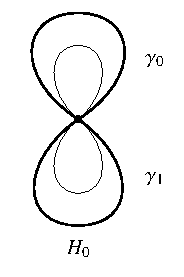
\includegraphics[width=.21\linewidth]{note6-fig-01.pdf}

\end{figure}

Therefore, \(\gamma_0\sim\gamma_1\), with fixed endpoints, if and only if \(\gamma_0+(-\gamma_1)\) is homotopic to a point.

\textit{Proof.}
Let \(H(t,s)\) be the deformation between \(\gamma_0\) and \(\gamma_1\). Then
\[
  \left.\gamma_0\right|_{[0,t]}(s)
  +H(s,t)
  +\left.(-\gamma_1)\right|_{[t,1]}(s)
  =:H'(t,s).
\]
Then \(H'\) shrinks \(\gamma_0+(-\gamma_1)\) to a point, one of its terminals. If \(H'(t,s)\) deforms a point to \(\gamma_0+(-\gamma_1)\), then
\[
  \left.\gamma_0\right|_{[t,1]}(s)
  +H'(t,s)
  +\left.\gamma_1\right|_{[0,t]}(s)
  =:H''(t,s).
\]
Thus, \(H''\) deforms \(\gamma_0\) to \(\gamma_0+(-\gamma_1)+(\gamma_1)\). We know \(\gamma_0+(-\gamma_1)\) deforms to a point, so \(\gamma_0+(-\gamma_1)+\gamma_1\sim\gamma_1,\)
and hence \(\gamma_0\sim\gamma_1\).


The following figures illustrate these deformations.

\[
  \gamma_0\sim\gamma_1
  \quad\Longleftrightarrow\quad
  \gamma_2+\gamma_1+(-\gamma_2)
  \qquad\text{for some }\gamma_2.
\]

\begin{figure}[htbp]
  \centering
  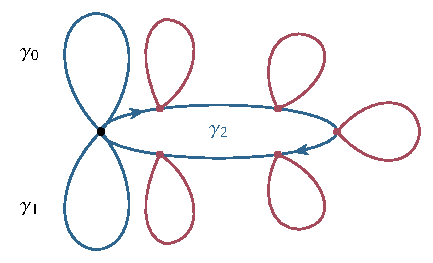
\includegraphics[width=.45\linewidth]{note6-fig-02.pdf}

\end{figure}

Here, \(\gamma_2\) is the curve formed by initial points in the family of curves belonging to the homotopy between \(\gamma_0\) and \(\gamma_1\), and
\[
  \gamma_2=H(t,0).
\]

\textbf{Remark.}
With this, if \(\gamma_0\sim\gamma_1\), as closed curves, then
\[
  \int_{\gamma_0}f=\int_{\gamma_1}f.
\]

Also,
\[
  \gamma_0\sim\gamma_1
  \quad\Longleftrightarrow\quad
  \gamma_0+(-\gamma_1)\sim\gamma_0(0).
\]

\begin{figure}[htbp]
  \centering
  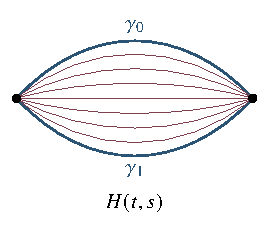
\includegraphics[width=.30\linewidth]{note6-fig-03.pdf}

\end{figure}

\begin{figure}[htbp]
  \centering
  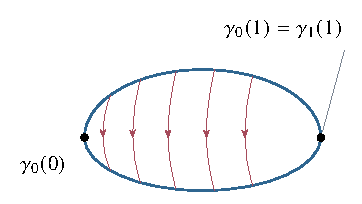
\includegraphics[width=.40\linewidth]{note6-fig-04.pdf}

\end{figure}

Here,
\[
  H'(t,s):=
  \left.\gamma_0(s)\right|_{[0,t]}
  +H(s,t)
  +\left.(-\gamma_1(s))\right|_{[t,1]}.
\]

\textbf{Remark.}
We denote a homotopy by \(H(t,s)\) to register the fact that \(t\) stands for the time variable in the event of deformation. Also, one must keep in mind the ways we collected curves from a homotopy and used curves to create a homotopy, thus justifying the


wording of Tool 21.

If \(U\) is connected and \(\gamma_0,\gamma_1:[a,b]\to U\) are two continuous curves, then there exists a continuous map
\[
  \gamma:[0,1]\times[a,b]\to U
\]
such that
\[
  \gamma(0,t)=\gamma_0(t),
  \qquad
  \gamma(1,t)=\gamma_1(t),
  \qquad t\in[a,b].
\]

\textit{Proof.}
The set \(U\) is path-connected. Let \(\gamma_2\) be the path from \(\gamma_0(0)\) to \(\gamma_1(1)\). Consider the curve
\[
  \gamma_1+\gamma_2+\gamma_0:[0,1]\to U.
\]
Without loss of generality, assume
\[
  \gamma_1:[0,\tfrac13]\to U,
  \qquad
  \gamma_2:[\tfrac13,\tfrac23]\to U,
  \qquad
  \gamma_0:[\tfrac23,1]\to U.
\]
We ``slide'' \(\gamma_1\) along the curve \(\gamma_1+\gamma_2+\gamma_0\) to reach \(\gamma_0\). Let \(\overline{\gamma}=\gamma_1+\gamma_2+\gamma_0\)
and define
\[
  \gamma_t:=\left.\overline{\gamma}\right|_{[t,\,1/3+t]}(s),
  \qquad 0\le t\le\frac23.
\]
After suitable normalization, one obtains what is needed.

\textbf{Remark.}
Because of these slides, which make the demand of a deformation rather trivial, we impose conditions such as \(H(s,0)=H(s,1)\qquad(\forall s),\)
which give us the notion of homotopy under closed curves, or the stronger condition that \(H(s,0)\) and \(H(s,1)\) are constants.

\subsection*{Tool 22 — Morera Technique}
We have seen two instances of this, one in the Schwarz Reflection Principle and the other in a variant of it. So, we shall briefly expound on it.

Suppose you are given a ``free'' homotopy \(H(t,s)\), a collection of curves \(\gamma_t(s):=H(t,s)\)
for a given \(t\). Let
\[
  H:[0,1]\times[0,1]\to\Omega,
\]
where \(\Omega\) is a domain. Then, by compactness of \([0,1]\times[0,1]\), we know \(H\) is uniformly continuous. Here we impose no particular conditions on \(H(t,0)\) and \(H(t,1)\). Let \(f\in C(\Omega)\). Then notice
\[
  \int_{\gamma_t(s)}f\sim\int_{\gamma_{t'}(s)}f
  \qquad\text{if }|t-t'|<\varepsilon.
\]

For every \(\varepsilon\), there exists \(\delta\) such that
\[
  |\gamma_t(s)-\gamma_{t'}(s)|<\varepsilon
  \quad\Longleftrightarrow\quad
  |t-t'|<\delta.
\]
Now note that
\[
  \int_{\gamma_t(s)}f
  :=\lim_{P}
  \sum_P f(\gamma_t(s_j^*))
  |\gamma_t(s_j)-\gamma_t(s_{j-1})|,
\]
where \(P\) is a partition of \([0,1]\). The restriction \(\left.f\right|_{H([0,1]\times[0,1])}\)
is also uniformly continuous, and so are \(\gamma_t(s)\) and \(\gamma_{t'}(s)\).

Given \(\varepsilon\),
\begin{align*}
  \left|\sum_{j=1}^n f(\gamma_t(s_j^*))
  |\gamma_t(s_j)-\gamma_t(s_{j-1})|\right|
  &\le
  \left|\sum_{j=1}^n
    \bigl(f(\gamma_t(s_j^*))-f(\gamma_{t'}(s_j^*))\bigr)
    |\gamma_t(s_j)-\gamma_t(s_{j-1})|\right| \tag{1}\\
  &\quad+
  \left|\sum_{j=1}^n f(\gamma_{t'}(s_j^*))
    |\gamma_{t'}(s_j)-\gamma_{t'}(s_{j-1})|\right| \tag{2}\\
  &\quad+
  \left|\sum_{j=1}^n f(\gamma_{t'}(s_j^*))
    |\gamma_{t'}(s_{j-1})-\gamma_t(s_{j-1})|\right|. \tag{3}
\end{align*}
Note that \((1)<\varepsilon/3\), \((2)<\varepsilon/3\), and \((3)<\varepsilon/3\) if the mesh size of the partition and \(|t-t'|\) are small enough. Hence,
\[
  \left|\sum_{j=1}^n f(\gamma_t(s_j^*))
  |\gamma_t(s_j)-\gamma_t(s_{j-1})|\right|
  <\left|\int_{\gamma_{t'}}f\right|+\varepsilon.
\]

Therefore,
\[
  \left|\int_{\gamma_t}f-
  \sum_{j=1}^n f(\gamma_t(s_j^*))
  |\gamma_t(s_j)-\gamma_t(s_{j-1})|\right|<\varepsilon,
\]
and
\[
  \left|\int_{\gamma_t}f\right|
  <\left|\int_{\gamma_{t'}}f\right|+\varepsilon
  \qquad(\forall\varepsilon).
\]
Thus,
\[
  \left|\int_{\gamma_t}f\right|
  =\left|\int_{\gamma_{t'}}f\right|.
\]
In particular, if one is \(0\), the other too is bound to be \(0\).

The technique is this: if \(f\in H(\Omega)\) and \(f\in C(\partial\Omega)\), then one can, as in the Reflection Principle, ``push down'' triangles past \(\partial\Omega\) and conclude that \(f\) can be extended.

\textbf{Exercise.}
Fill in the gaps, and remove the modulus.

% BLOG-PART
\subsection*{Tool 23 — Two-Ears Theorem}
Two-Ears Theorem (or the existence of a triangulation of any polygon).


\subsection*{Alexander Numbering Rule}
Refer to the statement in Tool 23. Draw the proof!

We first note that simple smooth curves locally look like rotated graphs. Let \(\gamma\) be a simple smooth curve, with
\[
  \gamma'(t_0)=re^{i\theta},
  \qquad
  \gamma:[a,b]\to\mathbb C,
  \qquad t_0\in(a,b).
\]
Then \(\gamma(t)=\gamma(t_0)+\gamma'(t_0)(t-t_0)+\psi(t)(t-t_0).\)
Consider
\begin{align*}
  \gamma'(t_0)(t-t_0)+\psi(t)(t-t_0)
  &=e^{i\theta}\left(r(t-t_0)+e^{-i\theta}(t-t_0)\psi(t)\right)\\
  &=e^{i\theta}\left(
    r(t-t_0)+\operatorname{Re}\bigl(e^{-i\theta}(t-t_0)\psi(t)\bigr)
    +i\operatorname{Im}\bigl(e^{-i\theta}(t-t_0)\psi(t)\bigr)
  \right).
\end{align*}
Let \(g(t)=e^{-i\theta}(t-t_0)\psi(t).\)
Notice that \(g'(t_0)=0\), as \(\psi(t_0)=0\), and hence
\[
  (\operatorname{Re}g)'(t_0)=0.
\]
Define locally
\[
  \varphi(t)=r(t-t_0)+\operatorname{Re}\bigl(e^{-i\theta}(t-t_0)\psi(t)\bigr).
\]
Then \(\varphi'(t_0)\ne0\), so \(\varphi\) is invertible locally. Let \(\varphi(t)=s\), so \(t=\varphi^{-1}(s)\), and set
\[
  f(s)=\operatorname{Im}(g)\circ\varphi^{-1}(s).
\]
Thus, locally, for \(\varepsilon\) small enough, we shall have the following to


be true:
\[
  \gamma([a,b])\cap B_\varepsilon(\gamma(t_0))
  =\left\{\gamma(t_0)+e^{i\theta}(s+if(s))
  \mid s\in(-c_\varepsilon,d_\varepsilon)\right\}.
\]

Let \(\gamma\) be the closed contour and \(\sigma\) the contour that has smooth transverse intersections with \(\gamma\) at the points
\[
  \{w_\ell\}_{\ell=1}^k.
\]
Notice that, to establish
\[
  W_\gamma(z_0)-W_\gamma(z_1)
  =\#\text{ left crossings}-\#\text{ right crossings},
\]
if one replaces \(\gamma\) and \(\sigma\) with approximate polygons \(\gamma_P\) and \(\sigma_P\), with the quantities \(W_\gamma(z_0)\), \(W_\gamma(z_1)\), the number of left crossings, and the number of right crossings preserved, then establishing the equality will complete the proof.

Let
\[
  \operatorname{dist}(\gamma,z_0)=\inf_t|\gamma(t)-z_0|=d_0,
  \qquad
  \operatorname{dist}(\gamma,z_1)=d_1,
\]
and let \(\delta=\min(d_0,d_1)\). We will stick to the \(\delta\)-neighborhood of \(\gamma\) and \(\sigma\), where
\[
  N_\delta(\gamma):=\{z\mid\operatorname{dist}(z,\gamma)<\delta\}.
\]
Denote this open set by \(\Omega\). Let \(\gamma^*\) and \(\sigma^*\) denote the images of \(\gamma\) and \(\sigma\). For every
\[
  \gamma(t_0)\in\gamma^*\setminus\{w_\ell\}_{\ell=1}^k,
\]
choose \(\varepsilon_{t_0}\) such that \(B_{\varepsilon_{t_0}}(\gamma(t_0))\subset(\sigma^*)^c.\)
Similarly for \(\sigma(t_0)\). For \(\{w_\ell\}_{\ell=1}^k\), choose \(\varepsilon_{w_\ell}\) so that in \(B_{\varepsilon_{w_\ell}}(w_\ell)\) the contours \(\gamma\) and \(\sigma\) look like rotated graphs. Note that the axioms of transverse intersection guarantee such an \(\varepsilon_{w_\ell}\) for every \(\ell\). Ensure all these balls lie in \(\Omega\).

Since \(\gamma^*\cup\sigma^*\) is compact, it has a finite cover. Let the balls covering \(\sigma^*\setminus\{w_\ell\}\) be \(\{\Sigma_i\}\), and those covering \(\gamma^*\setminus\{w_\ell\}\) be \(\{T_i\}\). The balls \(B_{\varepsilon_{w_\ell}}(w_\ell)=:B(w_\ell)\) must belong to the finite cover by the way such a cover is constructed. Repeat the


An important consequence of this is that every contour will be a concatenation of simple smooth curves, because the points in the set \(\{t\mid\gamma(t)=k,\ k\in\mathbb R^2\}\)
cannot accumulate in \([0,1]\), for these are locally like rotated graphs, which are one-manifolds, as ``non-loopy'' as an interval. Corollary: every polygon is a sum of simple polygons.


argument in the complex tube lemma, or assume without any further ``cherry-picking'' that the balls are successive. That is, there exists a partition
\[
  P=\{0=t_0<t_1<\cdots<t_n=1\}
\]
such that
\[
  \left.\gamma\right|_{[t_i,t_{i+1}]}
  \subset B_{\varepsilon_{t_i}}(\gamma(t_i))
  \cup B_{\varepsilon_{t_{i+1}}}(\gamma(t_{i+1})).
\]

One can similarly do so for \(\sigma\). Let us assume \(\{\Sigma_i\}\) and \(\{T_j\}\) are such consecutive balls. Exploiting the \(C^1\)-ness of \(\sigma\) and \(\gamma\), arrange matters so that

\[
  \arg\bigl(\gamma'_{\sigma(t)\to\sigma(t_i)}\bigr)
  =\arg\bigl(\sigma'(s_j)\bigr)+\varepsilon,
  \qquad \sigma(s_j)=w_\ell.
\]
Similarly for \(\sigma\). Let \(\Sigma_i\) and \(\Sigma_{i+1}\) be consecutive to \(B(w_\ell)\), with \(\sigma\), and let \(T_i\) and \(T_{i+1}\) be consecutive with \(\gamma\). Pick \(\sigma(t')\in\sigma^*\cap\partial B(w_\ell)\cap\Sigma_{i+1}\)
and, similarly, a point for \(\gamma\), and complete the polygonal paths. By construction, all those quantities will be preserved.

\textbf{Exercise.}
Finish the proof! Induct on the number of edges for a polygon via the invocation of the Two-Ears Theorem, as we did before, which would split
\[
  \gamma_P=\gamma_{P_1}+\gamma_{P_2}.
\]
Let the common edge be \(\gamma_{a\to b}\). If \(\sigma\) crosses \(+\gamma_{a\to b}\), every left crossing with \(\gamma_{P_1}\) is a right crossing with \(\gamma_{P_2}\), as the orientation reverses too. For a general closed polygon, simply write it as a finite concatenation of simple closed polygons, with the angle of the tangent varying smoothly.

\textbf{Remark.}
One reason this numbering rule is useful is that it tells us in which direction the interior lies. Recall the local description of a simple smooth curve. We have, as seen before,
\[
  \gamma([a,b])\cap B_\varepsilon(z_0)
  =\left\{z_0+e^{i\theta}(s+if(s))\mid s\in I_\varepsilon\right\}.
\]


There is one small thing that one must ensure, and that is that \(\gamma_P\) and \(\sigma_P\) preserve the crossing. For that, notice that once one obtains \(B(w_\ell)\), the set \((\gamma^*\cup\sigma^*)\setminus B(w_\ell)\)
is still compact.

Thus, the corresponding parts of \(\gamma^*\) and \(\sigma^*\) outside \(B(w_\ell)\) can be separated by \(T\) and \(\Sigma\). Now consider \(T\cap\Omega\) and \(\Sigma\cap\Omega\).


Perform suitable translations and rotations to get the graph as we know it. Let the \(x\)-axis be the line containing the derivative at \(t_0\) of \(\gamma\). Notice that the \(y\)-axis is perpendicular to the tangent at \(t_0\). Since the \(y\)-axis is unbounded, we know it contains both the interior and the exterior of \(\gamma\). Consider \(i\varepsilon\) and \(-i\varepsilon\). Let \(\gamma_{-i\varepsilon\to i\varepsilon}\) be the joining curve; clearly, \(\gamma_{-i\varepsilon\to i\varepsilon}\) is connected. Let \(\gamma\) be oriented anticlockwise. A simple connectedness argument tells us that \(i\varepsilon\) and \(-i\varepsilon\) lie in different components for all sufficiently small \(\varepsilon\). Just divide
\[
  \gamma_{-i\varepsilon\to i\varepsilon}\setminus\gamma^*
\]
into components and use the fact that \(\gamma\) is a graph, hence it cannot touch the \(y\)-axis more than once. Thus,
\[
  W_\gamma(i\varepsilon)-W_\gamma(-i\varepsilon)
  =\#\text{ left crossings}-\#\text{ right crossings}.
\]
But, after rotation,
\[
  \gamma'_{-i\varepsilon\to i\varepsilon}(0)
  =\lambda e^{i\pi/2},
  \qquad \lambda>0,
\]
where \(\gamma'(t_0)=re^{i\theta}\). This is true for all close translates of the \(y\)-axis. Set \(\varepsilon=\varepsilon'\). Then the interior of \(\gamma\) contains all points in \(D(z_0,\varepsilon)\) of the form
\[
  z_0+e^{i\theta}\bigl(s+i(f(s)+u)\bigr),
  \qquad u<\varepsilon.
\]
Draw!

\textbf{Remark.}
The previous remark essentially says that, if you traverse along the closed contour that is oriented anticlockwise, then the interior is to its left and the exterior is to the right. A symmetric statement can be made for clockwise orientation. Draw!

\subsection*{Tool 24 — Jordan Curve Theorem}
We stated before what it says, but what more it says is: if \(\operatorname{int}(\gamma)\subset U,\)
where \(U\) is some open set, then \(\gamma\) is null-homotopic in \(U\).

Here \(U\) is a domain. Therefore,
\[
  U\text{ is simply connected}
  \quad\Longleftrightarrow\quad
  \text{every }f\in H(U)\text{ is conservative}.
\]

\textit{Proof.}
Let \(z_0\in\operatorname{int}(\gamma)\), with \(\gamma^*\subset U\). If \(z_0\notin U\), then \(\frac{1}{z-z_0}\in H(U),\)
so
\[
  \int_\gamma\frac{1}{z-z_0}=0.
\]
But \(z_0\) is in the interior, so \(W_\gamma(z_0)\ne0\), a contradiction. Therefore, \(z_0\in U\), so \(\operatorname{int}(\gamma)\subseteq U.\)
Hence \(\gamma\) is contractible in \(U\), and \(U\) is simply connected.

\textbf{Remark.}
These singularity spikes ensure that there are no holes in the domain, for if there is one, they shall explode with a residue. So, if all smooth functions are conservative, in the sense that they have no residue, then ``there are no holes in \(U\).''

\paragraph{Observation.}
As in every star-shaped region, \(f\) has a primitive and is conservative; therefore, star-shaped regions are simply connected.

\textbf{Exercise.}
Using the ideas expounded in the remark following Alexander's Numbering Rule and the facts about \(W_\gamma(z)\), prove the Jordan Curve Theorem for polygonal paths, closed and simple. ``All the hard work has been done for this; one must merely connect the dots.''

\textbf{Remark.}
We do not need to invoke the Two-Ears Theorem to induct on the number of edges. If \(\gamma_P\) is a concave polygon oriented anticlockwise, let \(v\) be a vertex that has angle greater than \(\pi\) to the left of \(\gamma_P\), as in, towards the interior. Let the adjacent edges be \(e\) and \(f\), and extend


them until they meet some other point on the polygon \(\gamma_P\). This will split the polygon into two.

\[
  \gamma_1+\gamma_2=\gamma.
\]

\begin{figure}[htbp]
  \centering
  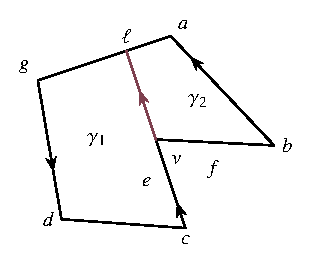
\includegraphics[width=.35\linewidth]{note6-fig-05.pdf}

\end{figure}

Regardless, it is worthy that we explore the proof of the Two-Ears Theorem. But, for our silly purposes, there is no need for any black boxes.

\textbf{Remark.}
One nice consequence of the above remark is the following. Now that we know how to define angles of a polygonal path, simple and closed, how do we do it? Pick a vertex, without loss of generality assume it is a base vertex, and let the edges meeting at \(v\) be \(e\) and \(f\). Let \(z_0\in e\), with \(z_0=\gamma(i)\), and \(z_1\in f\), with \(z_1=\gamma(j)\), where \(j>i\). Then separate \(v\) and \(\gamma|_{[i,j]}\). Let \(B_\varepsilon(v)\) be such that \(B_\varepsilon(v)\cap\gamma|_{[i,j]}=\varnothing.\)
Therefore, there exists a cone whose boundary is just a wedge of the polygon. Pick \(z_0\in e\) and \(z_1\in f\) such that \(|v-z_i|<\varepsilon\). If \(\gamma_{z_0\to z_1}\) is the canonical straight path, with \(\gamma_{z_0\to z_1}:[0,1]\to\mathbb C\), then
\[
  \left.\gamma_{z_0\to z_1}\right|_{(0,1)}
  \cap(\text{the polygon})=\varnothing.
\]
Thus, \(\left.\gamma_{z_0\to z_1}\right|_{(0,1)}\) lies entirely in the interior or the exterior. Based on that, define the angle to be \(\theta\) or \(2\pi-\theta\). Good.

Suppose all angles of the polygon are at most \(\pi\). We claim that the interior is convex. The argument to establish this is not that complicated. Consider translates


of the \(x\)-axis, \(i\alpha+\mathbb R\). Look at
\[
  (i\alpha+\mathbb R)\setminus\gamma^*.
\]
We intend to show that
\[
  \operatorname{int}(\gamma)\cap(i\alpha+\mathbb R)
\]
is a union of at most one interval. Thus, the same will be true, by suitable rotations, for any \(\alpha+e^{i\theta}\mathbb R\), which would yield that the segment joining two interior points is in the interior.

Without loss of generality, assume \(\operatorname{int}(\gamma)\cap\mathbb R\ne\varnothing\), and let \(\{I_j\}_{j\ge1}\) be its components, which are intervals. Pick two ``consecutive ones.'' Denote them by \(I_0\) and \(I_1\), with
\[
  I_0=(a_0,b_0),
  \qquad
  I_1=(a_1,b_1),
  \qquad a_0<b_0<a_1<b_1.
\]
Note that \([b_0,a_1]\) is not in \(\operatorname{int}(\gamma)\). One can argue that either of the following two situations can happen:

\begin{figure}[htbp]
  \centering
  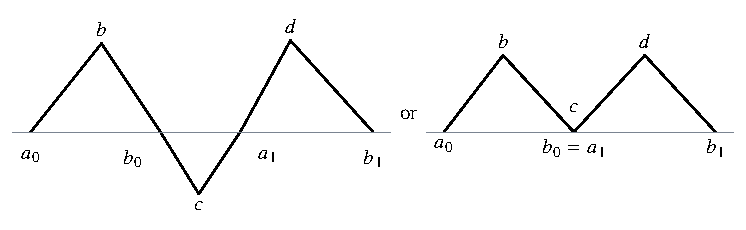
\includegraphics[width=.74\linewidth]{note6-fig-06.pdf}

\end{figure}

Using the meaning of angle which we just mentioned, one can conclude that the angle at \(c\) is greater than \(\pi\). So now one can have a topological view on convexity. We say that \(\gamma\), a simple closed curve, is convex if, for all \(z_0,z_1\in\operatorname{int}(\gamma)\), there exists a convex polygon \(\gamma_P\) such that
\[
  \gamma_P\cap\operatorname{ext}(\gamma)=\varnothing,
  \qquad
  z_0,z_1\in\operatorname{int}(\gamma_P).
\]

\paragraph{Digression.}
We claimed in the proof of Alexander's Numbering Rule that, by exploiting the \(C^1\)-ness of the curve, we can locally find a segment whose angle, with respect to slope, is the argument of the derivative of the point on the curve. Let us briefly justify it for the sake of completeness. Let \(\gamma(t_0)\) be in the interior of \([a,b]\), where \(\gamma:[a,b]\to\mathbb C\) is a smooth curve. Let \(\gamma'(t_0)=re^{i\theta}.\)
We know \(\gamma\) is locally a rotated graph, so by Rolle's theorem


there exists \(t'\in(a,b)\) such that \(\gamma'(t')=\frac{\gamma(b)-\gamma(a)}{b-a}.\)
Essentially, these arguments are the same. So, locally, if we establish the fact that
\[
  \arg(\gamma'(t_0))
\]
is continuous in \(t_0\), then we are done. This is easy to see because, locally around \(\gamma(t_0)\), a branch of the logarithm is defined, say in \(B_\varepsilon(\gamma(t_0))\). Now, in \(B_\varepsilon(\gamma(t_0))\), \(\frac{\gamma'(t)}{|\gamma'(t)|}\)
is continuous, so
\[
  \log_0\left(\frac{\gamma'(t)}{|\gamma'(t)|}\right)
\]
is continuous. Therefore, \(\arg(\gamma'(t))\) is continuous in \(B_\varepsilon(\gamma(t_0))\), which is precisely what we need.

\begin{figure}[htbp]
  \centering
  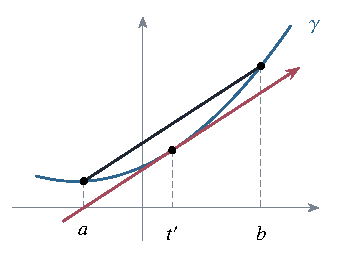
\includegraphics[width=.38\linewidth]{note6-fig-07.pdf}

\end{figure}

Let us work through the details; readers familiar with the argument may wish to skip ahead.

\subsection*{Jordan Curve Theorem (for simple closed polygonal paths)}
\textit{Proof.}
We saw before that, if \(\gamma_P\) is a simple smooth polygonal path, then \((\gamma_P^*)^c\) is a union of at least two components where \(W_{\gamma_P}\) is constant. Let \(\Omega\) be a region in \((\gamma_P^*)^c\). The function \(W_{\gamma_P}(z)\) is constant for \(z\in\Omega\). If \(W_{\gamma_P}(z)=k\), then \(W_{\gamma_P}\) attains \(k\) near \(\partial\Omega\), and hence \(W_{\gamma_P}\) attains \(k\) near \(\gamma_P\). Now, as was done in the argument of the remark following Alexander's Rule, conclude that, as \(z\) crosses the polygon, the winding number shifts by \(\pm1\). Hence, near \(\gamma_P([a,b])\), \(W_{\gamma_P}(z)\in\{k,k+1\}\)
in a neighborhood of \(z\) on \(\gamma_P\). Use the construction in the tube lemma to conclude that
\[
  W_{\gamma_P}(z)\in\{k,k+1\}
\]
in a neighborhood of \(\gamma_P\).


Now we know that \(W_\gamma(z)=0\) in the unbounded region, so \(W_\gamma(z)\in\{0,\pm1\}.\)
Two disjoint regions cannot have the same winding number, for near the boundary they switch by \(\pm1\). Therefore,
\[
  \{z\mid W_\gamma(z)=0\}
  \quad\text{and}\quad
  \{z\mid W_\gamma(z)=\sigma\},
  \qquad \sigma=\pm1,
\]
are connected. Now the claim of contractibility is already dealt with. QED.


\subsection*{Problems}
\emph{The motto of a problem is that it should make your life problematic.}

\begin{enumerate}
  \item Can you cover \(\mathbb R^2\) with curves joining \(z_1,z_2\in\mathbb R^2\) that are mutually disjoint, except that they have common endpoints?

  \item Let \(\gamma\) be a Jordan curve. Let \(f\in H(\operatorname{int}(\gamma))\) and \(g\in H(\operatorname{ext}(\gamma))\). Suppose that
  \[
    f\in C(\operatorname{int}(\gamma)\cup\gamma),
    \qquad
    g\in C(\operatorname{ext}(\gamma)\cup\gamma),
  \]
  so they extend continuously to their common boundary. Does there exist an entire function \(h\) such that \(h\) extends \(f\) and \(g\)?

  \item Let \(\gamma_1\) and \(\gamma_2\) be two Jordan curves, and let
  \[
    z_0\in\operatorname{int}(\gamma_1)\cap\operatorname{int}(\gamma_2)\ne\varnothing.
  \]
  If
  \[
    |z_0-\gamma_1(t)|<|z_0-\gamma_2(t)|,
  \]
  then does \(\gamma_1\) belong in \(\operatorname{int}(\gamma_2)\)?

  \item Given four discs around \(\{z_i\}_{i=1}^4\), say \(\{D_i\}_{i=1}^4\), with
  \[
    D_1\cap D_3\ne\varnothing,
    \qquad
    D_2\cap D_4\ne\varnothing,
    \qquad
    \overline{z_1z_3}\cap\overline{z_2z_4}\ne\varnothing,
  \]
  prove that if \(\gamma_{13}\) is a continuous curve joining \(z_1\) to \(z_3\), with
  \[
    \gamma_{13}^*\subset D_1\cup D_3,
  \]
  and similarly for \(\gamma_{24}\), then
  \[
    \gamma_{13}^*\cap\gamma_{24}^*\ne\varnothing.
  \]

  \item Let \(f:D\to\mathbb C\) be entire. If
  \[
    2|f'(0)|=\sup_{z,w\in D}|H(z)-H(w)|,
  \]
  then \(f\) is linear. (Shakarchi.)

  \item Using (4), or somehow devising a method, get a simple polygon homotopically close to a given simple closed curve. Let \(\gamma\) be any non-simple closed curve; again find a simple polygon homotopically close to it.
\end{enumerate}
% BLOG-CONTENT-END
\end{document}
